\documentclass[professionalfont]{beamer}
\usepackage{newtxtext}
\usepackage[heading = false, scheme = plain]{ctex}
\mode<presentation>{\usetheme{Warsaw}}
%\usecolortheme{dove}
\setbeamertemplate{footline}{}
\beamertemplatenavigationsymbolsempty
\addtobeamertemplate{navigation symbols}{}{%
    \usebeamerfont{footline}%
    \usebeamercolor[black]{footline}%
    \hspace{1em}%
    \insertframenumber/\inserttotalframenumber
}
\setbeamertemplate{caption}[numbered]
\usepackage{hyperref} 
\usepackage{bbm}
\usepackage{multirow}
\usepackage{amsmath}
\usepackage{listings}
\usepackage{natbib}
\usepackage{xcolor}
\usepackage{listings}
\usepackage{dsfont}
\def\R{{\mathbb R}}  %%
\def\E{{\mathbb E}}  %
\def\N{{\mathbb N}}  %%
\def\bx{\boldsymbol{x}}

\lstset{basicstyle=\tiny\ttfamily,
	numbers=left,
	breaklines=true,
	language=R,
}
\newcommand{\Rcode}[1]{\textcolor{blue}{\small \textrm{#1}}}
\newcommand{\Rout}[1]{\textcolor{green}{\small \textrm{#1}}}
\newcommand{\red}[1]{\textcolor{red}{#1}}
\newcommand{\green}[1]{\textcolor{green}{#1}}
\newcommand{\purple}[1]{\textcolor{purple}{#1}}
\newcommand{\blue}[1]{\textcolor{blue}{#1}}
\newcommand{\gray}[1]{\textcolor{gray}{#1}}




\title{第6讲:分类费率厘定 2 - 广义线性模型}
\author{高光远}
\institute{中国人民大学~统计学院}
\date{}
\begin{document}
%%title frame
\begin{frame}
	\titlepage
\end{frame}

\begin{frame}{主要内容}
	\tableofcontents
\end{frame}

%%table of contents
%\AtBeginSection[]
%{
%	\begin{frame}{}
%		\tableofcontents[currentsection]
%	\end{frame}
%}



%%normal frame
\begin{frame}{分类费率厘定模型: 确定性 VS 随机性}
\begin{itemize}
\item 从精算角度考虑, 费率因子需要和潜在损失相关.
\item 潜在损失观测不到, 只能看到经验损失(随机变量).
\item 利用经验损失数据, 检验费率因子的统计显著性.
\item 确定性模型无法进行统计检验, 需要建立随机性模型.	
\end{itemize}
\end{frame}
\begin{frame}{线性回归模型(linear regression, linear model)}
	$$Y_i\overset{ind}{\sim}\text{N}(\mu_i, \sigma^2)~\text{ with }~\mu_i=\beta_0+\beta_1x_{i1}+\cdots+\beta_dx_{id},\quad i=1,\ldots,n.$$ 
	基本假设:
	\begin{enumerate}
		\item $Y_i$ 互相独立.
		\item 方差不随期望的改变而变化.
		\item $Y_i$ 服从正态分布.
		\item $Y_i$ 的期望 $\mu_i$ 和协变量 $\bx_i$ 线性相关.
	\end{enumerate}
\end{frame}
\section{广义线性模型}
\begin{frame}{广义线性模型(generalized linear model, GLM)}
	
	$$Y_i\overset{ind}{\sim}\text{EDF}(\mu_i, \phi)\text{ with }g(\mu_i)=\eta_i=\beta_0+\beta_1x_{i1}+\cdots+\beta_dx_{id}, ~ i=1,\ldots,n.$$ 
	基本假设:
	\begin{enumerate}
		\item $Y_i$ 互相独立.
		\item 方差可以随期望的改变而变化.
		\item $Y_i$ 服从\red{指数型分布族(exponential dispersion family, EDF)}. 其\red{离散系数(dispersion)}为 $\phi$.
		\item $Y_i$ 的期望 $\mu_i$ 通过\red{连接函数(link function)} $g$ 和协变量 $\bx_i$ 线性相关.
	\end{enumerate}
\end{frame}
\subsection{指数型分布族}
\begin{frame}{自然参数和离散参数}
	指数分布族的概率密度函数可以表示为
	$$f(y_i;\theta_i,\phi)=\exp\left[\frac{y_i\theta_i-b(\theta_i)}{a(\phi)}+c(y_i,\phi)\right]$$
\begin{itemize}
\item $\theta_i$称为\red{自然参数(natural parameter)}, 不等于均值但和均值有关. 
\item $\phi$称为\red{离散参数(dispersion parameter)}, 不等于方差但和方差有关.
\item 每个观察值有\textbf{不同}的自然参数, 但有\textbf{相同}的离散参数.
\end{itemize}
\end{frame}
\begin{frame}{期望和方差}
	\begin{itemize}
	\item 函数 $a(\phi)$ 通常为 $\phi/\omega_{i}$, 其中 $\omega_i$ 表示 $y_i$ 的\red{权重}, 反映了 $y_i$ 的相对可信度.
	\item 通常, 当 $Y_i$ 表示第 $i$ 个风险集合的\textbf{平均索赔次数}时, 权重为该风险集合的\textbf{风险单位数}; 当 $Y_i$ 表示第 $i$ 个风险集合的\textbf{平均索赔金额}时, 权重为该风险集合的\textbf{赔付次数}.
	\item $Y_i$ 的期望为 \red{$\E(Y_i)=\mu_i=b'(\theta_i).$} \textbf{期望由自然参数唯一确定}, 和 $\phi$ 无关.
	\item 函数 $c(y_i,\phi)$ 和自然参数无关, 进而和期望无关. 因此也不会影响\textbf{回归参数} $\beta$ 的估计.
	\item $Y_i$ 的方差为$$\red{\text{Var}(Y_i)=a(\phi)b''(\theta_i)=\phi b''(\theta_i)/\omega_i}$$
	\item 定义\red{方差函数(variance function)}\red{$$V(\mu_i)=b''(\theta_i)/\omega_i$$}	
\end{itemize}
\end{frame}
\subsection{连接函数}
\begin{frame}
	\blue{注: 连接函数的选择不影响分布}.

	\begin{itemize}
	\item 期望 $\mu_i$ 通过\red{连接函数 $g$}, 与\red{线性预测项(linear predictor) $\eta_i$} 关联: 
	$$g(\mu_i)=\eta_i=\beta_0+\beta_1x_{i1}+\cdots+\beta_dx_{id}=\langle\beta,\bx_i\rangle.$$	
	\item \red{规范连接函数(canonical link function)} $$g_c(\mu_i)=\theta_i.$$
	即 $g_c$ 为 $b'$ 的逆函数. 当选用规范连接函数时, 自然参数等于线性预测项.
	\item 常见的规范连接函数有: \blue{恒等(正态), 对数(泊松), 倒数(伽马)}. 在logistic回归中, 常使用\blue{Logit连接函数},即
	$$g(\E(Y_i))=g(p_i)=\ln \frac{p_i}{1-p_i}=\langle\beta,\bx_i\rangle$$
	\end{itemize}
\end{frame}
\subsection{常见的指数型分布}
\begin{frame}\label{table}
	\begin{figure}
		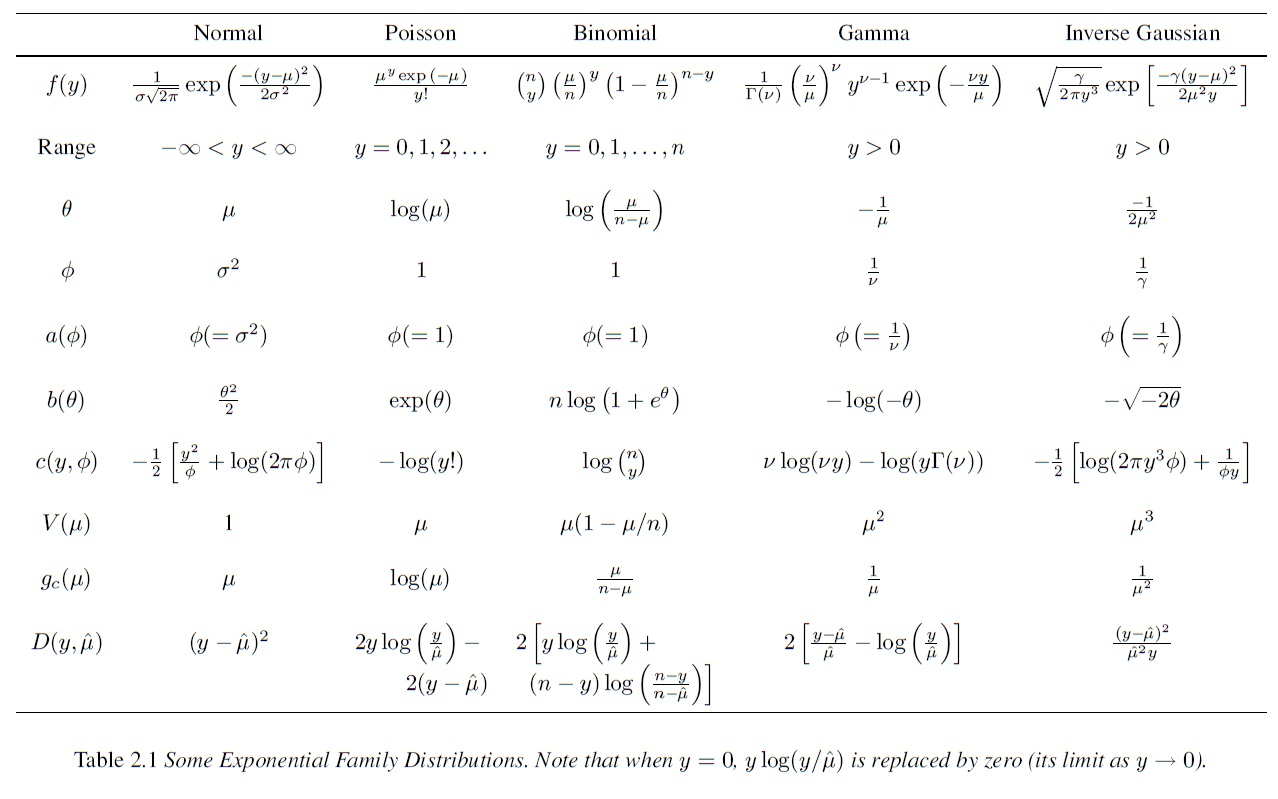
\includegraphics[width=\textwidth]{Plots/GLM.jpg}
	\end{figure}
\end{frame}
\section{参数估计}
\subsection{迭代加权最小二乘法}
\begin{frame}{Version 1}
	\begin{itemize}
		\item $g(\mu_i)$ 和协变量\textbf{线性相关}. 可以对 $g(\mu_i)$ 和协变量进行回归分析. 但是, $\mu_i$ 不知道, 暂用 $y_i$ 代替.
		\item 利用 Taylor 展开式, 可知 $g(Y_i)$ 的方差近似为
		\begin{equation}\label{delta}
		\text{Var}(g(Y_i))\approx \text{Var}(Y_i)g'(\mu_i)^2=\phi V(\mu_i)g'(\mu_i)^2.
		\end{equation}
		上述方法也称为\red{delta method}.
		\item 数据的离散度越大, 其可信度越低. 在 $g(Y_i)$ 和协变量的回归分析中, 需要使用\blue{加权最小二乘法(weighted least squares)}, 相对权重为\textbf{方差的倒数}:
		$$w_i=\frac{1}{V(\mu_i)g'(\mu_i)^2}.$$
		\item $\phi$ 为常数, 在相对权重中可以省略, 不影响参数估计.
	\end{itemize}
\end{frame}
\begin{frame}{Version 1}
	\red{迭代加权最小二乘法 1 (iterative re-weighted least squares, IRLS):}\\
	
	~
	
	给定初始 $\hat{\mu}_i^0=y_i$, 计算 $w_i^0=1/(V(\hat{\mu}^0_i)g'(\hat{\mu}^0_i)^2)$. 第 $t$ 步迭代为:
	\begin{enumerate}
		\item 以 $w_i^{t-1}$ 为权重, 通过如下加权最小二乘法求得 $\hat{\beta}^t$: 
		$$\underset{\beta}{\arg\min}\sum_{i=1}^n w_i^{t-1}\left(g(\hat{\mu}_i^{t-1})-\langle\beta,\bx_i\rangle \right)^2$$
		$\hat{\beta}^t$ 的解析解为 $\hat{\beta}^t=(X^TWX)^{-1}X^TWY$, 其中$X$为\red{设计矩阵(design matrix)}, $W=\text{diag}(w^{t-1}_1,\ldots,w^{t-1}_n).$
		\item 计算新的期望 $\hat{\mu}_i^t=g^{-1}(\langle\beta^t,\bx_i\rangle)$和新的权重:
		$$w_i^t=\frac{1}{V(\hat{\mu}_i^t)g'(\hat{\mu}_i^t)^2}.$$
	\end{enumerate}
	重复以上两步, 最终可以求出 $\beta$ 的极大似然估计.
\end{frame}
\begin{frame}{Version 2}
	假设有 $n$ 个观测值, 全样本可表示为 $\mathcal{D}=({\bx_i}, y_i)_{i=1:n}$. 可以推出其对数似然函数为
	$$l(\beta|\mathcal{D})=\sum_{i=1}^{n}\frac{y_i\theta_i-b(\theta_i)}{a(\phi)}+c(\phi,y_i)=\sum_{i=1}^{n}\frac{\omega_i\left[y_i\theta_i-b(\theta_i)\right]}{\phi}+c(\phi,y_i)$$
	上式关于$\beta_j$求偏导
	\begin{equation}\label{irls1}
	\frac{\partial l}{\partial \beta_j}=\frac{1}{\phi}\sum_{i=1}^n\omega_i\left(y_i\frac{\partial\theta_i}{\partial \beta_j}-b'(\theta_i)\frac{\partial\theta_i}{\partial\beta_j}\right)=\frac{1}{\phi}\sum_{i=1}^n\omega_i\left[y_i-b'(\theta_i)\right]\frac{\partial\theta_i}{\partial \beta_j}
	\end{equation}
		其中, 
		$$\frac{\partial \theta_i}{\partial \beta_j}=\frac{\partial \theta_i}{\partial \mu_i}\frac{\partial \mu_i}{\partial \beta_j}=\frac{1}{b''(\theta_i)}\frac{\partial \mu_i}{\partial \beta_j}.$$
\end{frame}
\begin{frame}{Version 2}

	式 \eqref{irls1} 进一步等于
	\begin{equation}
	\frac{\partial l}{\partial \beta_j}=\frac{1}{\phi}\sum_{i=1}^n\frac{y_i-b'(\theta_i)}{b''(\theta_i)/\omega_i}\frac{\partial\mu_i}{\partial \beta_j}=\frac{1}{\phi}\sum_{i=1}^n\frac{y_i-\mu_i}{V(\mu_i)}\frac{\partial\mu_i}{\partial \beta_j}
		\end{equation}
	所以, $\beta$ 的极大似然估计, 为以下方程组的解
	\begin{equation}\label{irls2}
	\sum_{i=1}^n\frac{y_i-\mu_i}{V(\mu_i)}\frac{\partial\mu_i}{\partial \beta_j}=0 ~ \forall ~ j
	\end{equation}
		如果式 \eqref{irls2} 中 $V(\mu_i)$ 为已知,且和 $\beta$ 独立, 则式\eqref{irls2}对应于一个\blue{非线性加权最小二乘法}, 其目标函数为: 
		\begin{equation}\label{irls3}
		\mathcal{S}=\sum_{i=1}^n\frac{(y_i-\mu_i)^2}{V(\mu_i)}
		\end{equation}
\end{frame}

\begin{frame}{Version 2}

迭代加权最小二乘法 2 (iterative re-weighted least squares, IRLS)\\

~

给定初始 $\hat{\beta}^0$, 计算 $V(\hat{\mu}^0_i)=V(g^{-1}(\langle\hat{\beta}^0,\bx_i\rangle))$. 第 $t$ 步迭代为:
\begin{enumerate}
	\item 以$1/V(\hat{\mu}_i^{t-1})$为权重, 通过非线性加权最小二乘法 \eqref{irls3} 求得$\hat{\beta}^t$. 
	\item 计算 $V(\hat{\mu}_i^t)=V(g^{-1}(\langle\hat{\beta}^t,\bx_i\rangle))$. 
\end{enumerate}
 重复以上两步, 最终可以求出 $\beta$ 的极大似然估计.
\end{frame}
\subsection{离散参数的估计}
\begin{frame}{Pearson 方法}
定义\red{Pearson统计量}为
$$\red{X^2=\sum_{i=1}^n\frac{(y_i-\hat{\mu}_i)^2}{V(\hat{\mu}_i)}}$$
当样本足够大, 近似地, 
$$\frac{X^2}{\phi}\sim\chi^2_{n-d-1}.$$
所以, 离散参数 $\phi$ 的估计为
$$\red{\hat{\phi}_P=\frac{X^2}{n-d-1}}.$$
此方法为R估计离散参数的方法.
\end{frame}
\begin{frame}{偏差(deviance)}
\begin{itemize}
\item 定义\red{偏差统计量(deviance, deviance statistics)}为
$$\red{D(\hat{\beta}_{full},\hat{\beta})=2\phi[l(\hat{\beta}_{full})-l(\hat{\beta})]}.$$
其中$\hat{\beta}_{full}$为\blue{饱和模型(saturated model)}的参数估计. 
\item 在饱和模型中, 一个因变量对应一个期望参数$\mu_i$, 共有$n$个(回归)参数. 可以推出, \blue{参数的极大似然估计为$\hat{\mu}_i=y_i$}. 
\item 因此, 计算 $\phi l(\hat{\beta}_{full})$ 时, 只需要知道因变量的值, 不需要知道协变量的值,  $l(\hat{\beta}_{full})$ 也常记作 $l(\boldsymbol{y})$. 
\item 符号$\hat{\beta}_{full}$主要为了和$\hat{\beta}$对比, 并没有实际意义.
\item 偏差统计量类似于\red{sum of squared error (SSE)}, 反映了拟合优度. 可以证明,在高斯分布条件下, Deviance=SSE.
\item Deviance和SSE的缺点是\blue{对过拟合不敏感}.
\end{itemize}
\end{frame}
\begin{frame}{偏差法}
	\begin{itemize}
	\item  定义\red{scaled-偏差统计量(scaled deviance)}为
$$\red{D^*(\hat{\beta}_{full},\hat{\beta})=D(\hat{\beta}_{full},\hat{\beta})/\phi=2[l(\hat{\beta}_{full})-l(\hat{\beta})]}.$$
\item 关于常见指数型分布的偏差统计量, 请参考第 \ref{table}页
	\item 可以证明$D(\hat{\beta}_{full},\hat{\beta})$和$\phi$无关, $D^*(\hat{\beta}_{full},\hat{\beta})$和$\phi$有关. (作业)
	\item 若模型正确且样本足够大, $D^*(\hat{\beta}_{full},\hat{\beta})=D(\hat{\beta}_{full},\hat{\beta})/\phi$ 近似服从 $\chi^2_{n-d-1}$. 所以, 离散参数的另外一种估计方法为:
	$$\red{\hat{\phi}_D=\frac{D(\hat{\beta}_{full},\hat{\beta})}{n-d-1}}.$$
	\item 在线性回归中, 上式可写为:
	$$\hat{\sigma}^2=\text{MSE}=\frac{\text{SSE}}{n-d-1}$$
	\end{itemize}
\end{frame}
\subsection{极大似然估计的大样本性质}
\begin{frame}
定义\red{费雪信息(Fisher information matrix)}如下
\begin{equation}
\mathcal{I}(\beta)=\left(-\E\left[\frac{\partial^2l(\beta)}{\partial\beta_l\beta_r}\right]\right)_{0\le l,r\le d+1}
\end{equation}
当样本足够大时, 可以证明
\begin{equation}\label{fisher}
\blue{\hat{\beta}\sim \text{N}(\beta, \mathcal{I}(\beta)^{-1})}
\end{equation}
可以看到极大似然估计为\red{无偏估计}. 
\end{frame}
\begin{frame}
根据\eqref{fisher}可以做\red{假设检验(Hypothesis testing)}, 如$$H_0: \beta_r=0.$$ 
在索赔频率回归模型中, 上面的假设检验即检验第 $r$ 个分类变量和索赔频率的相关性是否\blue{统计显著}.
\end{frame}
\section{预测和检验}
\subsection{预测}
\begin{frame}{预测}
	\begin{itemize}
	\item 	$Y_i$ 的期望为 $\mu_i$. $\mu_i$ 为常数, 可通过$\hat{\beta}, \bx_i$进行\red{估计}
	$$\hat{\mu}_i=g^{-1}(\langle\hat{\beta},\bx_i\rangle).$$
	\item 通过 Taylor 展开, $\hat{\mu}_i$的\red{估计方差}为:
	\begin{equation}\label{delta2}
	\text{Var}(\hat{\mu}_i)\approx\frac{\bx_i^T\text{Var}(\hat{\beta})\bx_i}{g'(\hat{\mu}_i)^2}.
	\end{equation}
	\item 随机变量 $Y_i$ 也可以通过 $\hat{Y}_i=\hat{\mu}_i$ 进行\red{预测}. 其\red{预测均方误差(mean square error of prediction, MSEP)}为
	\begin{equation}\label{MSEP}
	\E\left[\left(Y-\hat{Y}\right)^2\right]=\left(\E[Y]-\E[\hat{Y}]\right)^2+\text{Var}(\hat{Y})+\text{Var}(Y).
	\end{equation}
	其中, 右边第一项称为\blue{偏差 (bias)}, 第二项称为\blue{估计方差 (estimation variance)}, 最后一项称为\blue{过程方差 (process variance)}.
	\end{itemize}
\end{frame}
\subsection{检验}
\begin{frame}{Pearson residuals}
	定义\red{Pearson残差}为
	$$\epsilon^P_i=\frac{y_i-\hat{\mu}_i}{\sqrt{V(\hat{\mu}_i)}}.$$
	定义scaled-Pearson残差为
	$$\epsilon^{SP}_i=\frac{y_i-\hat{\mu}_i}{\sqrt{\phi V(\hat{\mu}_i)}}.$$
	可知
	$$X^2=\sum_{i=1}^n\left(\epsilon_i^P\right)^2$$
\end{frame}
\begin{frame}{Deviance residuals}
	定义\red{偏差残差(deviance residuals)}为
	$$\epsilon^D_i=\text{sign}(y_i-\hat{\mu}_i) \sqrt{2\phi[l_i(\hat{\beta}_{full})-l_i(\hat{\beta})]}.$$
其中, $l_i$表示第$i$个样本的对数似然函数.\\
	定义scaled-偏差残差(scaled-deviance residuals)为
	$$\epsilon^{SD}_i=\text{sign}(y_i-\hat{\mu}_i)\sqrt{2[l_i(\hat{\beta}_{full})-l_i(\hat{\beta})]}.$$
	可知
	$$D(\hat{\beta}_{full},\hat{\beta})=\sum_{i=1}^n\left(\epsilon_i^D\right)^2$$
	在理想的残差图中, 残差应该在原点两侧对称随机分布, 并没有明显的模式. 否则, 需要重新考虑\textbf{分布}的选取, 或者\textbf{连接函数}的选取.
\end{frame}
\begin{frame}{正态检验}
	根据参数极大似然估计的大样本性质:
	\begin{equation*}\label{fisher2}
	\hat{\beta}\sim \text{N}(\beta, \mathcal{I}(\beta)^{-1})
	\end{equation*}
	可以给出每个参数的置信区间, 进而进行假设检验. 如 $H_0: \beta_r=0$ 或 $H_0: \beta_r=2$.
\end{frame}
\begin{frame}{似然比检验}
	检验模型中某些协变量和因变量的相关性是否统计显著.
	$H_0: \beta_1=\ldots=\beta_p=0$ for $1\le p<d$
	\begin{enumerate}
		\item 计算完整模型的scaled-偏差统计量$D^*(\hat{\beta}_{full},\hat{\beta})$
		\item 计算在 $H_0$ 下模型的scaled-偏差统计量$D^*(\hat{\beta}_{full},\hat{\beta}_{H_0})$
		\item 定义检验统计量
		\begin{equation}\label{chi}
		\red{D^*(\hat{\beta},\hat{\beta}_{H_0})=D^*(\hat{\beta}_{full},\hat{\beta}_{H_0})-D^*(\hat{\beta}_{full},\hat{\beta})=2[l(\hat{\beta})-l(\hat{\beta}_{H_0})]}
		\end{equation}
		\item  在 $H_0$ 下, $D^*(\hat{\beta},\hat{\beta}_{H_0})\sim\chi^2_{p_1-p_0}$.  在 $\alpha$ 的显著水平下, 如果$$D_{H_0}\geq\chi^2_{p_1-p_0}(1-\alpha),$$
		拒绝 $H_0$. 这里 $p_1=d+1$ 为完整模型$\beta$参数的个数, $p_0=d+1-p$ 为 $H_0$ 模型$\beta$参数的个数. $p_1-p_0=p$.
	\end{enumerate}
\end{frame}
\begin{frame}{正态检验 VS 似然比检验}
	\begin{itemize}
		\item 正态检验类似于线性回归中的 $t$ 检验, 每次只能检验一个协变量的显著性.
		\item 似然比检验类似于线性回归中的 $F$ 检验, 可以同时检验多个协变量的显著性, 也可以检验 \blue{$H_0: \beta_s=\beta_t$}.
	\end{itemize}
\end{frame}
\section*{}

\begin{frame}
	\begin{enumerate}
		\item 阅读教材4.4.
		\item 自测课后习题. 
		\item 证明式 \eqref{delta}, 式 \eqref{delta2}, 式 \eqref{MSEP}.
		\item 证明$D(\hat{\beta}_{full},\hat{\beta})$和$\phi$无关, $D^*(\hat{\beta}_{full},\hat{\beta})$和$\phi$有关. 
\item 证明$D(\hat{\beta}_{full},\hat{\beta})\geq0$. 
	\end{enumerate}
\end{frame}

\end{document}